\chapter{Algorithms for Equations of Motion integration}

\section{Harmonic oscillator}
Implement the Velocity Verlet algorithm. Consider the harmonic oscillator:
\begin{equation}
	\begin{aligned}
		\dot q &= p \\
		\dot p &= -\omega^2 q
	\end{aligned}
	\label{eq111}
\end{equation}
Check the energy conservation, plotting $(E(t) - E_0)/E_0$ vs $t$, $E_0$ being the initial total energy and the discrepancy with the analytical solution as a function of time. Verify that the Velocity Verlet is stable (i.e. it follows the analytical solution) for $\omega \Delta t < 2$ checking a few values of $\omega$.

\textbf{\\ Resolution \\}

The system in Eq. \ref{eq111} can be quite easily integrated with standard analysis; the solution, given a set of initial conditions $(q_0, p_0)$ reads:
\begin{equation}
	\begin{aligned}
		q(t) &= q_0 \cos(\omega t) + \frac{p_0}{\omega}\sin(\omega t) \\
		p(t) &= p_0 \cos(\omega t) - q_0\omega\sin(\omega t)
	\end{aligned}
\end{equation}
For the sake of simplicity, we are going to simulate trajectories that started in $t=0$ at $q_0 = 1, p_0 = 0$, so that the equations of motion can be simplified:
\begin{equation}
	\begin{aligned}
		q(t) &= \cos(\omega t) \\
		p(t) &= - \omega\sin(\omega t)
	\end{aligned}
\end{equation}
The Hamiltonian for such a system is (remember $m = k = 1$):
\begin{equation}
	\mathcal{H} = \frac{1}{2}\omega^2 q^2 + \frac{1}{2}p^2
\end{equation}
and $\mathcal{H}$ is conserved because this is a Hamiltonian system. 

A generic EOM integrator would compute a sequence of states $(q_0 = 1, p_0 = 0; q_1, p_1; q_2, p_2, ..., q_n, p_n)$, at discrete time-steps $\Delta t$. In particular, the Velocity Verlet works by updating positions $q_i$ and momenta $p_i$ according to:
\begin{equation}
	\begin{aligned}
		q(t+\Delta t) &= q(t) + \dot q(t)\Delta t + \frac{1}{2}F(q(t))\Delta t^2 \\
		p(t+\Delta t) &= p(t) + \frac{1}{2}(F(q(t)) - F(q(t+\Delta t)))\Delta t
	\end{aligned}
\end{equation}
where $F(q(t))$ is the force acting at time $t$ (which should be a function of positions only). It's quite easy to show that the error that one makes when using Velocity Verlet is, at each time steps, of the order of $O(\Delta t^3)$ (local error). However, to fully integrate the equations of motion on a finite interval $	[0, T]$, we have to repeat the local algorithm $O(\frac{1}{\Delta t})$, so that errors can build up and the final global error should be on the order of $O(\Delta t^2)$. 

A nice property of Velocity Verlet, despite it being a 2nd order integrator, is that it displays symplectic properties. This implies that, although the integrator proceeds in finite timesteps, it always conserves a quantity in phase-space (called the shadow Hamiltonian $\mathcal{H}'$). This is a desirable property, especially in physics where most of the ODEs possess a Hamiltonian structure and the conserved quantity (the Hamiltonian itself) has a direct and fulfilling interpretation, i.e. the total mechanical energy of the system. Other integration schemes (for example, Runge-Kutta methods) are higher-order integrators, hence the error they make is usually smaller, but they fail to correctly preserve the energy over long time windows. 

A minimal snapshot of the implemented code for the Velocity Verlet (VV) algorithm is shown here:
\begin{lstlisting}[language=python]
	def velocity_verlet_step(q, p, dt, a, omega):
		p += 0.5 * a * dt       # Update velocity by half step
		q += p * dt		        # Update position by full step
		a_t_dt = -omega**2 * q  # Compute acceleration at new position
		new_a = a_t_dt          # Cache the force, so it only has to be computed once
		p += 0.5 * a_t_dt * dt  # Update velocity by another half step
		return q, p, new_a
	
	def run(omega, dt, T, q=1, p=0):
		steps = int(T / dt)
		a_t = -omega**2 * q  		# Initial acceleration
		q_traj = np.zeros(steps)
		p_traj = np.zeros(steps)
		for i in range(steps):
		q, p, a_t = velocity_verlet_step(q, p, dt, a_t, pmega)
		q_traj[i] = q
		p_traj[i] = p
		return q_traj, p_traj
\end{lstlisting}
The harmonic oscillator integrated trajectories are displayed in phase space in Fig.\ref{fig:phasespaceHO} and in a timeplot in Fig.\ref{fig:trajHO} having set $\omega = 1$. As expected, the trajectory in phase space closely resembles a circle centered in the origin with radius $\omega=1$. Furthermore, the oscillatory nature of the solutions is nicely reproduced by the algorithm. 
\begin{figure}
	\centering
	\includegraphics[scale=0.5]{./FIG/phase_space_trajectory.pdf}
	\caption{\textit{On the left, phase space representation of the simulated trajectories when $\Delta t = 0.01$ integrating from $t=0$ up to $T = 120$. On the right, a close up view of a smaller portion of the plane region, where the granularity of the algorithm becomes clearer (and the arrow of time is color coded.)}}
	\label{fig:phasespaceHO}
\end{figure}
\begin{figure}
	\centering
	\includegraphics[scale=0.4]{./FIG/qp_trajectory.pdf}
	\caption{\textit{Velocity Verlet integrated curves for $\omega q(t)$ and $p(t)$ (on the right, a closer and zoomed view to better see the discrete points). Overall, the algorithm has found a seemingly convincing trajectory reproducing the typical oscillations of the physical problem. It looks like a small bias is present in all steps, but this will be better studied later on}}
	\label{fig:trajHO}
\end{figure}

As stated before, the VV algorithm is supposed to be symplectic, i.e. it has to conserve a phase-space observable which is allegedly close enough to the actual Hamiltonian of the problem. To verify whether this property truly holds in our specific case, we study the percentage variation of the empirical energy $E_n = \frac{1}{2}\omega^2 q_n^2 + \frac{1}{2}p_n^2$ compared to the true actual energy $\mathcal{H} = \mathcal{H}(q_0, p_0) = \frac{1}{2}\omega^2 = E_0$ throughout time in Fig.\ref{fig:energyHO}. The characteristic percentage deviation from the actual value $E_0$ and oscillates back and forth in time around a typical value $-1.25 \times 10^{-5}$ with a period approximately half of the natural period of the coordinates trajectory. In particular, the integrator always underestimate the true energy of the system, but within a reasonable bounded interval. This is a good sign and confirm the symplectic nature of the algorithm, meaning that no energetic drift will appear during the numerical integration of the equations of motion. 
\begin{figure}
	\centering
	\includegraphics[scale = 0.4]{./FIG/energy_conservation.pdf}
	\caption{\textit{Percentage variation of integrated energy $E(t)$ with respect to the constant true value $E_0$. The plot clearly shows that the integrator always underestimate the energy by an oscillating amount bounded by $\max \Delta E \approx -2.5\times 10^{-5}E_0$. Overall, the symplectic nature of the VV algorithm is confirmed. }}
	\label{fig:energyHO}
\end{figure}
Another way to verify whether the VV has correctly integrated Eq.\ref{eq111} is to simply plot the variation with respect to the analytical form of $q(t), p(t)$: this is done in Fig.\ref{fig:difftrajHO}\footnote{If the coordinate $q$ is of order $1$, then $p$ is usually of order $\omega$, so we normalize $p(t)/\omega$ to get realistic results.}. The variation for both $q$ and $p$ is of the order of $1\%$, hence we can be satisfied with the algorithm's output.
\begin{figure}
	\centering
	\includegraphics[scale = 0.4]{./FIG/deviation_analytical.pdf}
	\caption{\textit{Relative variation of $q(t), p(t)$ with respect to the true analytical curves as a function of time. Similarly to Fig.\ref{fig:energyHO}, the deviation oscillates back and forth around $0$ and stays bounded within $\approx 1\%$.}}
	\label{fig:difftrajHO}
\end{figure}
\paragraph{Maximum deviation} 
Based on the trajectories in Fig.\ref{fig:difftrajHO}, we can extract the maximum deviation for both $q$ and $p$ (denoted as $\Delta q, \Delta p$) and interpret it as the typical error incurred by the Velocity Verlet (VV) algorithm when the time-step is set to $\Delta t = 0.01$. 
We expect that decreasing $\Delta t$ will lead to smaller errors, although at a higher computational cost: to verify this behavior, we compute the associated error across a range of $\Delta t$ values (Fig.\ref{fig:errorHO}). 
The Verlet algorithm is found to be stable up to a threshold value $\Delta t^\star$ satisfying $\omega \Delta t^\star = 2$; beyond this limit, the algorithm becomes unstable, yielding divergent trajectories (left panel of Fig.\ref{fig:errorHO}).

\begin{figure}
	\centering
	\includegraphics[scale = 0.5]{./FIG/max_deviation_vs_deltat}
	\caption{\textit{Algorithmic errors (intended as maximum deviations of $q(t), p(t)$ from their theoretical curves) vs time-step $\Delta t$, keeping $\omega=1$ fixed. The left plot highlights the existence of a threshold at $\Delta t = \frac{2}{\omega}$ above which the error skyrockets and the integrator completely fails. The rightmost plot can be used to infer the scaling behavior of the error with respect to $\Delta t$, $\Delta q \propto O(\Delta t^2)$ (a typical property of a 2nd order integrator such as VV).}}
	\label{fig:errorHO}
\end{figure}
\begin{figure}
	\centering
	\includegraphics[scale = 0.5]{./FIG/max_deviation_vs_omega.pdf}
	\caption{\textit{Algorithmic errors (intended as maximum deviations of $q(t), p(t)$ from their theoretical curves) vs $\omega$, this time keeping $\Delta t=0.01$ fixed. The same critical value $\omega = \frac{2}{\Delta t}$ can be seen from a different perspective (no points over that value since overflows errors hindered the numerical integration). A scaling behavior $O(\omega^3)$ emerges. }}
	\label{fig:errorHO2}
\end{figure}

Furthermore, the right panel of the same figure highlights another key feature of the algorithm: the characteristic scaling of the error with respect to the time-step $\Delta t$ (at fixed $\omega$). Since VV is a second-order integrator, we expect a scaling behavior of $\Delta q, \Delta p \sim O(\Delta t^2)$, which is precisely what the numerical results confirm (at least up to the critical $\Delta t^\star$).

The same plot can be realized by keeping $\Delta t $ fixed to $\Delta t = 0.01$ and letting $\omega$ vary (Fig.\ref{fig:errorHO2}). Again, we observe a critical threshold when $\omega = \frac{2}{\Delta t}$ above which the Python interpreter failed because of a overflow error, suggesting the trajectory diverged and exploded to infinity. The scaling of the error is now $O(\omega^3)$.



\section{Lennard-Jones fluid in the NVE ensemble}
The purpose of this section is to simulate the dynamical evolution of a system composed of $N = 200$ interacting particles using MD techniques to infer thermodynamical quantities such as the internal energy or structural properties like the radial distribution function. The simulation is carried on using a dedicated and powerful software called LAMMPS, which enables us to instantiate and inspect highly-customizable Molecular-Dynamics simulation. 

LAMMPS can be readily used in the terminal given a script file is provided. The script file should contain all the details that the LAMMPS MD engine will need to run the computations. An instructive section of the script that I've used is reported here for the sake of completeness:

\begin{itemize}
	\item{Step 1: Initialization}. In this section, we tell LAMMPS the geometric properties of our simulation: 
	
	\begin{lstlisting}
		# 1) Initialization
		units lj
		dimension 3
		atom_style atomic
		boundary p p p
			
		# 2) System definition
		region simbox block 0 6.85824 0 6.85824 0 6.85824
		create_box 1 simbox
		create_atoms 1 random 200 34134 simbox overlap 0.3\end{lstlisting}
	This portion of the script will instruct LAMMPS to generate a $3D$ box with periodic boundary condition whose size is $L = 6.85824$. This value of $L$ was chosen such that the final volume of the simulation $V = L^3$ will yield the target numerical density $\rho = 0.62$. The last line will make LAMMPS generate particles at random trying the avoid overlaps within $0.3$ units from the center of each molecule.\footnote{Spatial units are rescaled in terms of molecular sizes, as usual in MD simulation}
	
	\item{Step 2: settings} This section will define the parameters associated with the pairwise potential making particles interact. In this case, we're going to use the Lennard-Jones potential:
	\begin{equation}
		V(r) = 4\epsilon \Bigl(\Bigl(\frac{\sigma}{r}\Bigr)^{12}-\Bigl(\frac{\sigma}{r}\Bigr)^6\Bigr)
	\end{equation}
	units are rescaled in such a way that $\sigma = 1$ and $\epsilon=1$.
	\begin{lstlisting}
		# 3) Settings
		mass 1 1.0
		pair_style lj/cut 4
		pair_coeff 1 1 1.0 1.0
		pair_modify shift yes\end{lstlisting}
	The second line allows us to select the cut-off radius of the potential, i.e. the distance over which particles don't feel any type of interaction. In this report, we are going to examine what happens to the moleculars systems when $r_{cut} =4, 3, 2.5, 2^{1/6}$. The last value was chosen because it is precisely the stable equilibrium point for the pair-wise Lennard-Jones potential, where particles feel no net force. In practice, when $r_{cut} = 2^{1/6}$ we only retain the repulsive part of the Lennard-Jones potential, reducing the problem to a simple hard-sphere simulation that we already encountered in the previous chapter.
	
	The last line \texttt{pair\_modify shift yes} is crucial: if we simply cut the LJ potential for $r < r_{cut}$ and assume $V(r)=0$ for $r > r_{cut}$, then we'd introduce a steep potential discontinuity in $r_c$ (in general $V_{LJ}(r_{cut}\neq0)$). This translates in an impulsive non-conservative force that will break the energy conservation condition. To make sure this doesn't happen, we have to add a constant energy term to the LJ potential to ensure continuity in $r=r_{cut}$, which is what we do with that last line in the script. A more detailed discussion of this problem is discussed and illustrated in Fig.\ref{fig:LJplot}
	
	\item{Step 3: Minimization}
	During the generation phase, LAMMPS will simply place molecules in a random fashion, uniformly within the volume $L^3$. However, especially when the numerical density is large, there's a high chance that two particles are created very close one to each other, experiencing extremely large and potentially unstable forces. To avoid this problem, we will let LAMMPS run a pre-processing phase whose main goal is to find a spatial configuration that minimizes the (potential) energy:
	\begin{lstlisting}
		minimize 1.0e-6 1.0e-6 1000 10000\end{lstlisting}
	Note that this is not yet the numerical integration section
	
	\item{Step 4: Thermalization}
	As of now, we have only prepared the state trying to find a non-overlapping spatial configuration where the potential energy is stable. We still haven't dealt with the kinetic part of the system, as the velocities of the particles were left untouched. Since we want to run a energy-conserving simulations where $T =1$, we should sample the particles' velocities according to the correct Maxwell-Boltzmann distribution (ensuring no net drift). An alternative way to initialize the particles momenta is to introduce with LAMMPS a temporary thermostat that will bring the temperature of the system up to the desired value:
	\begin{lstlisting}
		fix equil all langevin 1.0 1.0 0.1 99999
		fix integrate all nve
		thermo 100
		run 5000
		# Now we can turn off the thermostat
		unfix equil
		unfix integrate\end{lstlisting}
	At the end of this stage, we can remove the thermostat. By now, all velocities should be initialized in such a way that $T = 1$.
	\item{Verlet integration}
	We have correctly initialized the spatial configurations and the velocities of the system: we can now run the MD simulations selecting the timestep $\Delta t$ and the total integration time:
	\begin{lstlisting}
		# 5) Finally, run the MD simulation
		reset_timestep 0
		fix mynve all nve
		timestep 0.005
		run 1000000\end{lstlisting}
	Note that the line \texttt{fix mynve all nve} will use Verlet algorithm under the hood, so we expect energy to be conserved.
\end{itemize}
\begin{figure}
	\centering
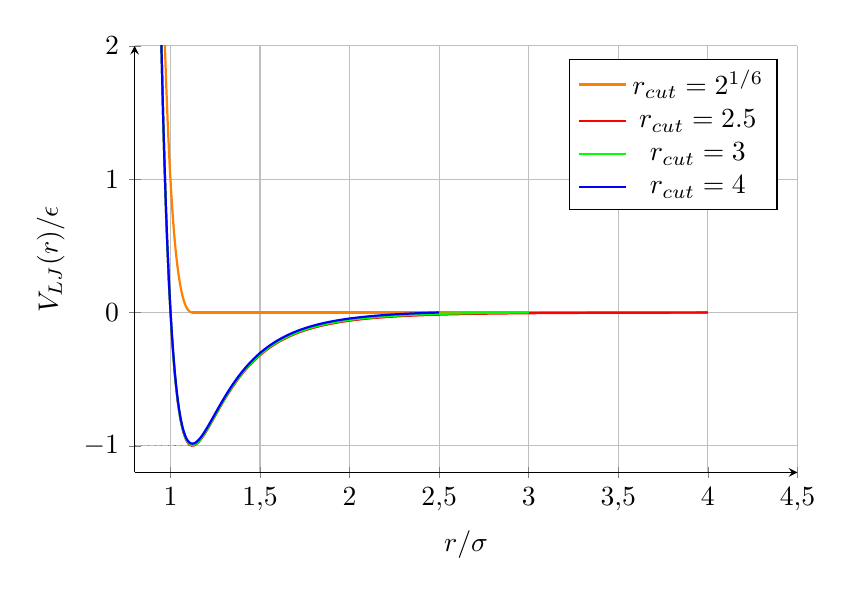
\begin{tikzpicture}
	\begin{axis}[
		% Impostazioni Assi
		axis lines = left,
		xlabel = {$r / \sigma$},
		ylabel = {$V_{LJ}(r) / \epsilon$},
		% Limiti del grafico
		xmin = 0.8, xmax = 4.5,
		ymin = -1.2, ymax = 2.0,
		% Stile
		grid = major,
		width = 10cm,
		height = 7cm,
		legend pos = north east,
		/pgf/number format/.cd,
		use comma,
		1000 sep={}
		]
		
		\addplot [
		domain=1.122:4, 
		samples=200, 
		color=orange, 
		thick,
		]
		{0};
		
		\addplot [
		domain=0.85:4, 
		samples=200, 
		color=red, 
		thick,
		]
		{4*(x^(-12) - x^(-6))};
		\addlegendentry{$r_{cut} = 2^{1/6}$}
		
		\addplot [
		domain=0.85:3, 
		samples=200, 
		color=green, 
		thick,
		]
		{4*(x^(-12) - x^(-6)) + 0.0055};
		\addlegendentry{$r_{cut} =2.5$}
		
		\addplot [
		domain=0.85:2.5, 
		samples=200, 
		color=blue, 
		thick,
		]
		{4*(x^(-12) - x^(-6))+0.016};
		\addlegendentry{$r_{cut} = 3$}
		
		\addplot [
		domain=0.85:1.122, 
		samples=200, 
		color=orange, 
		thick,
		]
		{4*(x^(-12) - x^(-6)) + 1};
		\addlegendentry{$r_{cut} = 4$}
		

		
		% Linea verticale per r_cut = 4

		\draw [gray, dotted] (axis cs:0.8, -1) -- (axis cs:1.122, -1);
		
	\end{axis}
\end{tikzpicture}
\caption{\textit{Lennard-Jones potential cut at different distances $r_{cut}$. Note that cutting the potential at small $r$ will introduce a discontinuity in the $V(r)$, i.e. a delta-shaped instantaneous force which has no physical relevance and can inject spurious energy absorption into the system. To counterbalance this problem, one should just add a constant term $+V_{LJ}(r_{cut})$. This procedure has little effect on $r_{cut} = 4, 3, 2.5$ where $V(r_{cut}) \approx 0$ but must be implemented on $r_{cut} = 2^{1/6}$ where $V_{LJ}(2^{1/6}) = -1$. The resulting potential is also called Weeks-Chandler-Andersen (WSA) potential in the scientific community}}
\label{fig:LJplot}
\end{figure}
\subsection{Energy conservation}
Let $E_0$ be the initial energy of the system:
$$
E_0 = K_0 + V_0 = \sum_i \frac{1}{2}p_i^2(t=0) + \sum_{i\neq j} V_{LJ}(r_{ij}(t=0))
$$
where the $p_i(t=0)$ were sampled from the Maxwell-Boltzmann at temperature $T=1$ thanks to the thermostat phase in LAMMPS and the configuration was chosen at random while keeping sufficient distance between the molecules. The time evolution of the total energy is reported in Fig. \ref{fig:energyLJ} for $\rho = 0.62$ and $\rho = 0.4$. Along with the relative energy variation, Fig. \ref{fig:energyLJ} also displays the behavior of the temperature $T$ as a function of time. 

Overall, the VV integrator has produced valid trajectories and the energy has approximately stayed constant: in the worst scenario (when $r_{cut}=1.12\approx 2^{1/6}$), the relative variation with respect to $E_0$ was about $\approx 0.1\%$, which is a solid result and an usually acceptable value when performing MD simulations. Furthermore, one has to consider that the simulation was run until $10^6$ steps were reached: other more sophisticated integration schemes (e.g. Runge-Kutta methods) would have probably better approximated the system during the initial steps but would have yielded a noticeable and unacceptable energy drift over the course of $1$ million time-steps. 

Let us now analyze individual results. When $r_{cut} = 4$, the energy-conservation plot is surprisingly nice for both $\rho = 0.62$ and $\rho = 0.4$: small energy fluctuations of the order of $10^{-4}E_0$ can still be appreciated, but no overall energy drift is detected. When $\rho = 0.62$ and $r_{cut}=3.0$, we observe an interesting phenomena: the system experiences a small positive drift during the first half of the simulation3 and then stabilizes around a fixed plateau (up to some small fluctuations). This is both a good and a bad news: during the first steps, the integrator has injected a small and unphysical amount of energy into the system, breaking energy conservation. However, this trend eventually came to an end and the integrator regained its ability to maintain the energy stationary. Strictly speaking, to obtain stable and robust results, we should have only considered the system in its stationary phase (even though here the energy is different than the one we started with); however, the drift in energy is well below the acceptable threshold, so we included all the time evolution in the analysis to come. The same reasoning goes for the most unstable configurations with $r_{cut} = 2.5$ and $r_{cut} = 2^{1/6}$, where a stationary phase (meaning no drift, just small fluctuations) is harder to find and multiple drifting phases coexist. Still, the overall energy variation is well bounded within $\approx 0.1\%$, hence we can proceed with our analysis.


Another interesting aspect to study is the time evolution of the temperature $T$ which can (and should) vary over time, since we are in a microcanonical ensemble, not in a canonical one. Overall, we expect a temperature fluctuating around the fixed value $\langle T \rangle=1$, and now the entity of the fluctuations is macroscopic ($\approx 10/20 \%$) and has relevant physical properties. Fig.\ref{fig:energyLJ} partially agrees with this theoretical analysis in all cases, but there are small deviations from the expected behavior of $T(t)$. For example, computing the average $T$ over all MD samples, we always observe a slightly different value with respect to $\langle T \rangle = 1$, suggesting a leak (or an injection) of kinetic energy from (into) the system (Table \ref{table:table2}). This is, however, to be expected: from the analysis of the energy $E(t)$ over time, we observed small inconsistencies due to the imperfect nature of the algorithm. Those spurious and unphysical energy leaks/injections have direct effect on the kinetic energy, and, consequently, on the temperature $T$. As long as we don't measure huge deviations from $\langle T \rangle = 1$, we can safely use those results to build robust analysis.

\begin{table}
	\centering
		\begin{tabular}{|c|c|c|}
		\hline
		$r_{cut}$ &  Average $\bar T$ & St Dev $\sigma_T$\\
		\hline
		$4$ &  1.038 & 0.0320 \\
		$3.5$  &  1.0464 & 0.0320\\
		$2.5$  &  1.0700 & 0.0323\\ 
		$1.122$ & 1.0462 & 0.0282\\
		\hline
	\end{tabular}
		\begin{tabular}{|c|c|c|}
		\hline
		$r_{cut}$ &  Average $\bar T$ & St Dev $\sigma_T$\\
		\hline
		$4$ &  0.9685 & 0.0453\\
		$3.5$  &  0.9775 & 0.0447\\
		$2.5$  &  1.0413 & 0.0394\\ 
		$1.122$ & 1.0493 & 0.0204\\
		\hline
	\end{tabular}
	\caption{\textit{Average temperature and associated standard deviation at different values of $r_{cut}$ when $\rho = 0.62$ (left) and $\rho = 0.4$ (right). }}
	\label{table:table2}
\end{table}

\begin{figure}
	\centering
	\includegraphics[scale = 0.4]{./FIG/energyLJ_0_62.pdf}
	\includegraphics[scale = 0.4]{./FIG/energyLJ_0_40.pdf}
	\caption{\textit{Energy and temperature plots at different cut-off radius $r_{cut}$ when $\rho = 0.62$ (first two rows) and $\rho = 0.4$ (last two rows). The time-step was set to $\Delta t = 0.005$ and the number of steps is $10^6$. Overall, the energy deviations and the average temperature are well behaved and bounded. In the temperatures plots, the average $\bar T$ is represented with a dashed line and the standard deviation with a solid band.}}
	\label{fig:energyLJ}
\end{figure} 


\subsection{Potential and kinetic energy}
Provided our simulations have faithfully conserved the total energy $E(t)$ within reasonable bounds, we can start analyzing other physical properties of interest like the potential and kinetic energy. The resulting histograms for those observables (normalized per number of particles) are reported in Fig.\ref{fig:histoKU}.
\begin{figure}
\centering
\includegraphics[scale = 0.4]{./FIG/hist_kin_pot_LJ_0_62}
\includegraphics[scale = 0.4]{./FIG/hist_kin_pot_LJ_0_4}
\caption{\textit{Histograms for the kinetic energy per particle (on the left) and the potential energy per particle (on the right) at various cut-off distances when $\rho = 0.62$ (top band)} and $\rho = 0.4$ (bottom band)}
\label{fig:histoKU}
\end{figure}
Let us first derive how the kinetic energy histogram should look like. By invoking the equipartition theorem, we can write:
\begin{equation}
	\langle K\rangle = \frac{3}{2}Nk_B \langle T \rangle
\end{equation}
for monoatomic gases. Note this is absolutely independent of the potential shape, even more so from the cut-off radius. Since we work with $k_B = 1$ and $T=1$, we should see a kinetic energy per particle $K = 1.5$ \textit{independent of $r_{cut}$}. The kinetic energy histograms in Fig. \ref{fig:histoKU} are compatible with this computation and closely resemble gaussian distributions, but their average values is slightly different from the expected $K = 1.5$, especially for $\rho = 0.62$ when all the $4$ simulations tend to overestimate the correct value of $K$. I believe this is again a matter of numerical instability of the integrator and a direct consequence of the total temperature drift that was commented in the previous subsection: in fact, one can easily see that the worst results for the kinetic energy (that is, the farthest from $K = 1.5$) were obtained when $\rho = 0.62$ and $r_{cut} = 2.5$, the same set of parameters that yielded the worst temperature average in Table \ref{table:table2}. The average kinetic energies are, however, perfectly correlated with the average measured temperature, so that those two anomalies are intimately linked (recall $\langle k \rangle = \frac{3}{2} \langle T \rangle$).

%Another reason to believe that those mismatches are essentially due to the integrator per se and not on some physically relevant property is that they are more evident when the system is more crowded, i.e. when $\rho = 0.62$. Every time a particle is moved

Now let us analyze the behavior of the potential energy. When $r_{cut} = 4,3,2.5$ the attractive well of the Lennard-Jones potential is kept (Fig.\ref{fig:LJplot}) and allows for the formation of persistent inter-molecules bonds, resulting in negative potential energies per particles. The largest $r_{cut}$ is, the more we keep of the attractive portion of the potential and the final average potential energy per particle gets more and mode negative (until an asymptotic value is reached for $r_{cut} = \infty$). However, if we truncate the potential at $r_{cut} = 2^{1/6}$, we completely remove the attractive property of the Lennard-Jones potential and the molecules simply behave by repelling each other if they get too close one to another. This type of truncation, also called \textit{WCA potential}, is a continuous version of the hard sphere model where particles don't interact with each other apart from the exclusion volume repulsion. The potential energy now becomes positive (but this is simply due to the constant added term we already discussed) and, most importantly, close to $0$, precisely what we would expect from a hard sphere model

Observing Fig.\ref{fig:histoKU}, the average potential energy approaches $0$ but does not vanish completely. This occurs because the WCA potential is steep yet differentiable; consequently, particles with sufficiently high kinetic energy can temporarily penetrate the distance $r<1$, resulting in a significant gain in potential energy. This effect becomes much more evident as the system density increases, since the crowdedness and the reduced free volume forces particles to interact more frequently with their neighbors.

\subsection{Radial distribution function}
Finally, we analyze the radial distribution function $g(r)$ of the system, computed via molecular dynamics simulations using LAMMPS. The results are plotted in Fig.\ref{fig:LJrdf}. 
By setting the cutoff radius to $r_{cut} = 4$, we essentially capture the full range of the interaction; consequently, we observe the typical oscillatory behavior characteristic of the Lennard-Jones potential, where peaks alternate with minima. This structural ordering indicates that the fluid possesses significant short-range order. The first sharp peak corresponds to the nearest-neighbor shell, located approximately at the distance where the Lennard-Jones potential reaches its minimum (around $r \approx 2^{1/6}\sigma$). This implies that particles tend to cluster at this energetically favorable distance.  Subsequent peaks represent further coordination shells (next-nearest neighbors). However, as $r$ increases, these oscillations progressively vanishes and $g(r)$ converges to $1$. This decay implies the absence of long-range order, confirming that the system is indeed in a fluid phase where spatial correlations vanish over long distances but are fundamental at small scales.
\begin{figure}
	\centering
	\includegraphics[scale = 0.4]{./FIG/rdf_LJ_0_62.pdf}
	\includegraphics[scale = 0.4]{./FIG/rdf_LJ_0_40.pdf}
	\caption{\textit{Radial distribution function $g(r)$ for the Lennard-Jones model at different cut-off radius when $\rho =0.62$ (above) and $\rho = 0.4$ (below) }}
	\label{fig:LJrdf}
\end{figure}
On the contrary, when $r_{cut} = 2^{1/6}$ the system essentially behaves as a hard sphere model: hence, the radial correlation completely vanishes when $r>2^{1/6}$ since particles only interact thanks to the excluded volume. Note that the curve for $r_{cut} = 2^{1/6}$ is in agreement with the one in Fig.\ref{fig:g(r)} 

For intermediate cut-off radius, the radial distribution curves are similar to the one obtained for $r_{cut} = 4$, since we are still retaining most of the initial Lennard-Jones potential. This is particularly evident for $\rho = 0.62$ but becomes less noticeable when $\rho = 0.4$, where the three different curves (the one for $r_{cut} = 4, 3, 2.5$) start to become diverge one from another. This is because when $\rho = 0.6$, the typical distance between molecules is $\frac{1}{\rho} \approx 1.6$. It's highly improbable the a pair of particle is found at a distance much larger than $1.6$, hence the effect of a cutoff is negligible (as long as $r_{cut} >> \frac{1}{\rho}$). When $\rho = 0.4$, the typical distance is now $2.5$, hence with our choice of cut-off radius we should start to observe some discrepancies in the three curves. As expected, the larger the value of $r_{cut}$ the higher the first peak gets, since larger $r_{cut}$ implies more attraction between particles (and more short-range structure)